\documentclass[../main.tex]{subfiles}

\begin{document}

\appendix
\renewcommand\chaptername{Appendix}  % This is to change 'chapter' to 'appendix' in the header

% Uncomment these lines (up to \chapter) to suppress appendix name in the header
% Uncommenting leaves just chapter name and number, eg: "Appendix A"

% \fancypagestyle{plain}{
%     \fancyhead[LE,RO]{\chaptername \ \thechapter}
% }


% \fancypagestyle{appendix}{
%     \fancyhead[LE,RO]{\chaptername \ \thechapter}
% }

% \pagestyle{appendix}

\chapter{Backtest Visualization} \label{appendix:backtest_visualization}


\section*{SETF Restructuring Turnover}

See Figure~\ref{fig:appendix_backtest:setf_restructuring_turnover} on Page~\pageref{fig:appendix_backtest:setf_restructuring_turnover}.


\section*{Portfolio Rebalancing Turnover}

See Figure~\ref{fig:appendix_backtest:portfolio_rebal_turnover} on Page~\pageref{fig:appendix_backtest:portfolio_rebal_turnover}.


\section*{Portfolio Return}

See Figure~\ref{fig:appendix_backtest:portfolio_return} on Page~\pageref{fig:appendix_backtest:portfolio_return}.

\section*{Sharpe Ratio}

See Figure~\ref{fig:appendix_backtest:sharpe_ratio} on Page~\pageref{fig:appendix_backtest:sharpe_ratio}.


\newpage
\begin{sidewaysfigure}
    \centering
    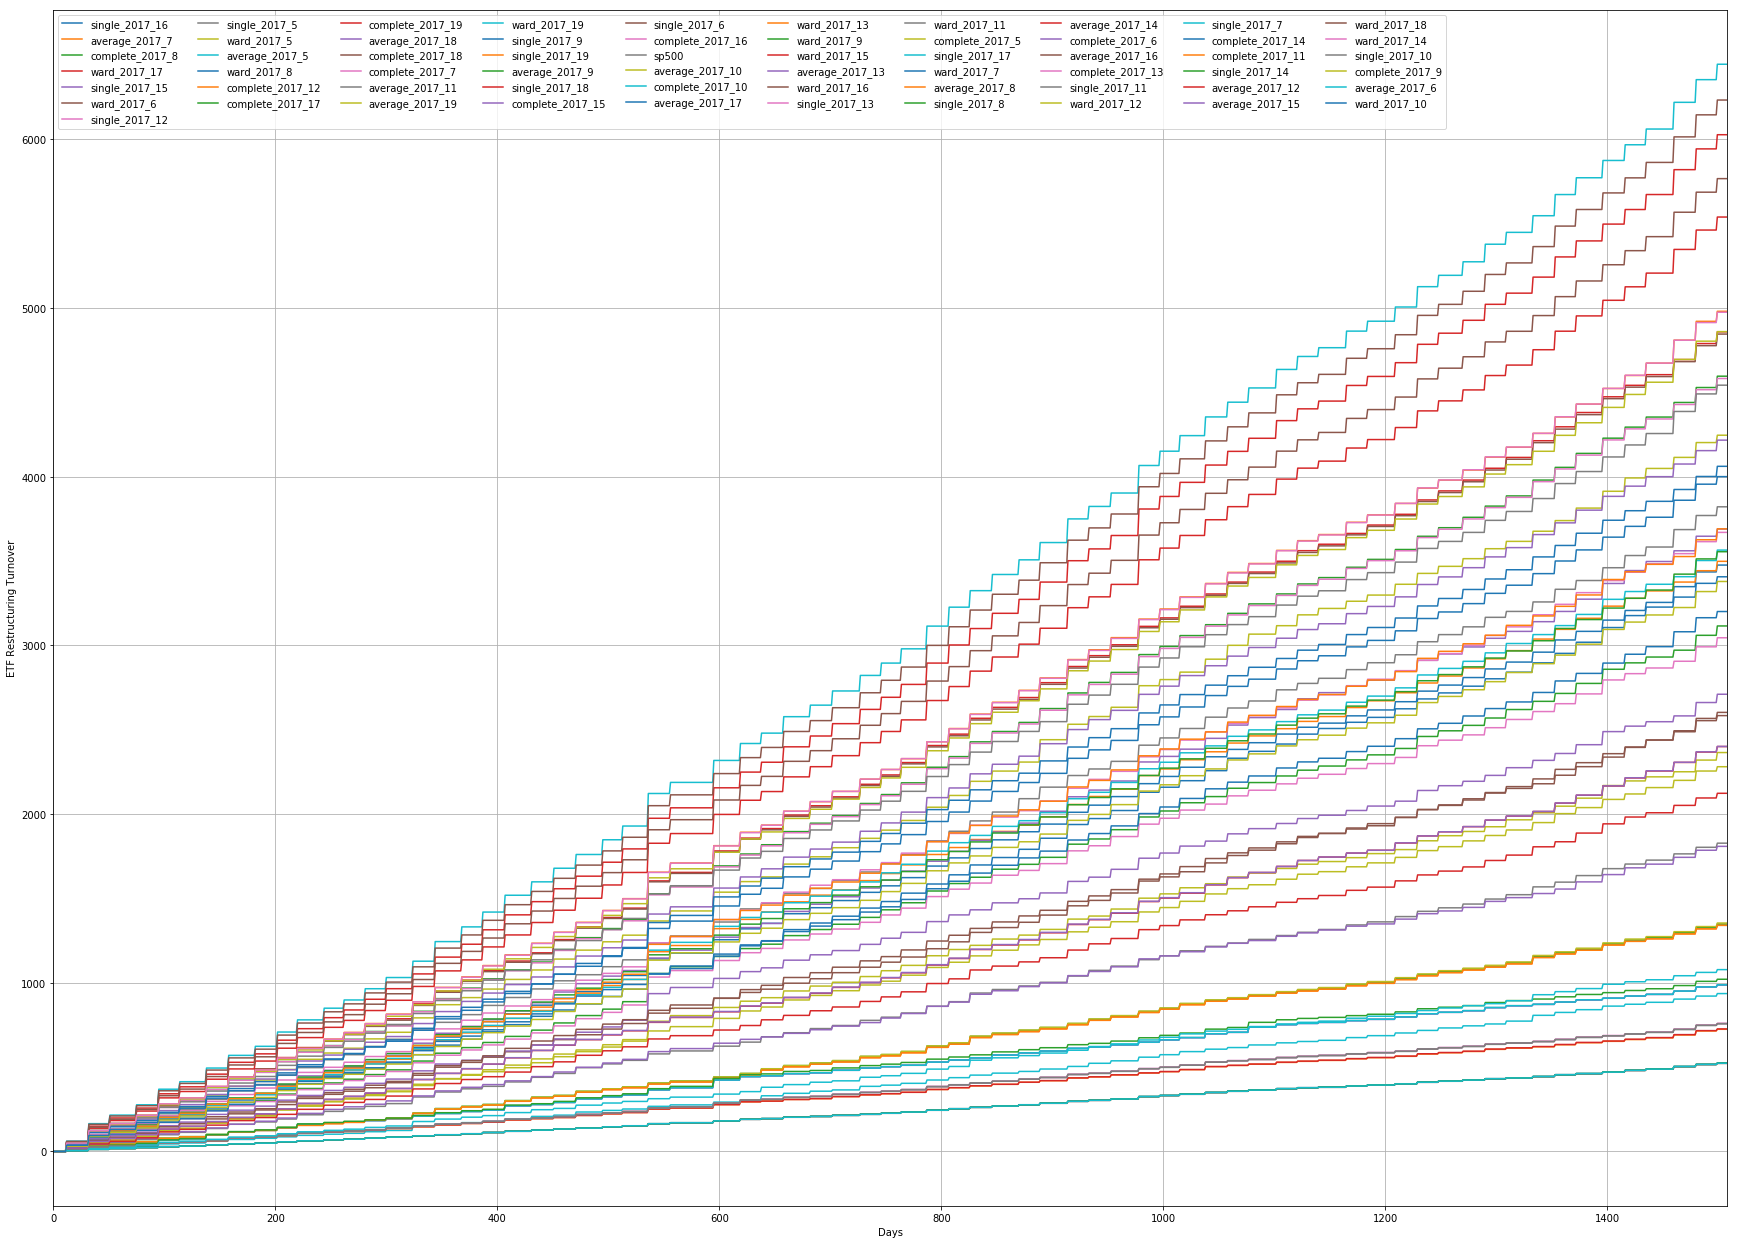
\includegraphics[width=\linewidth]{images/all_setf_restructuring_turnover.png}
    \caption{Cumulative SETF restructuring turnover for 60 candidate learned sector universes.}
    \label{fig:appendix_backtest:setf_restructuring_turnover}
    \addcontentsline{toc}{section}{SETF Restructuring Turnover}
\end{sidewaysfigure}

\newpage
\begin{sidewaysfigure}
    \centering
    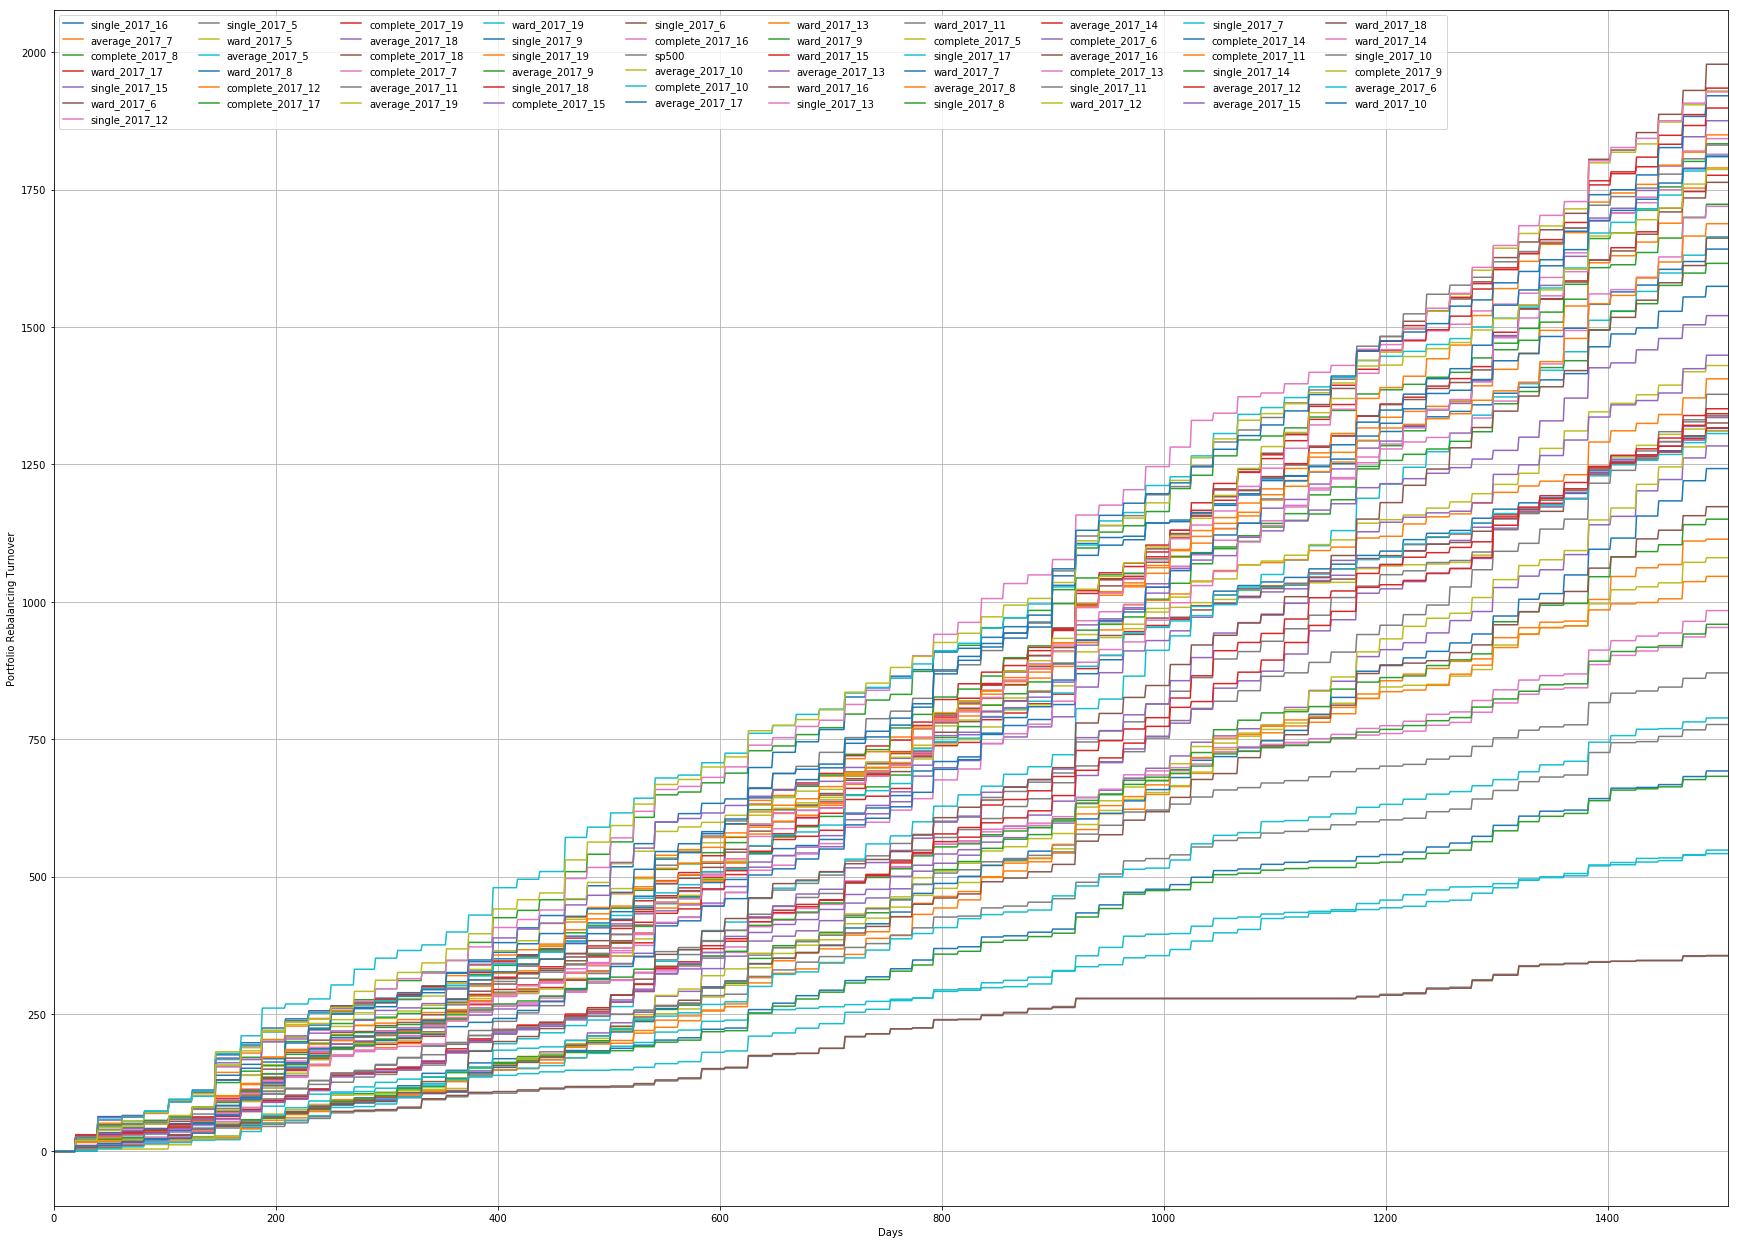
\includegraphics[width=\linewidth]{images/all_portfolio_rebalancing_turnover.png}
    \caption{Cumulative portfolio rebalancing turnover for 60 candidate learned sector universes.}
    \label{fig:appendix_backtest:portfolio_rebal_turnover}
    \addcontentsline{toc}{section}{Portfolio Rebalancing Turnover}
\end{sidewaysfigure}

\newpage
\begin{sidewaysfigure}
    \centering
    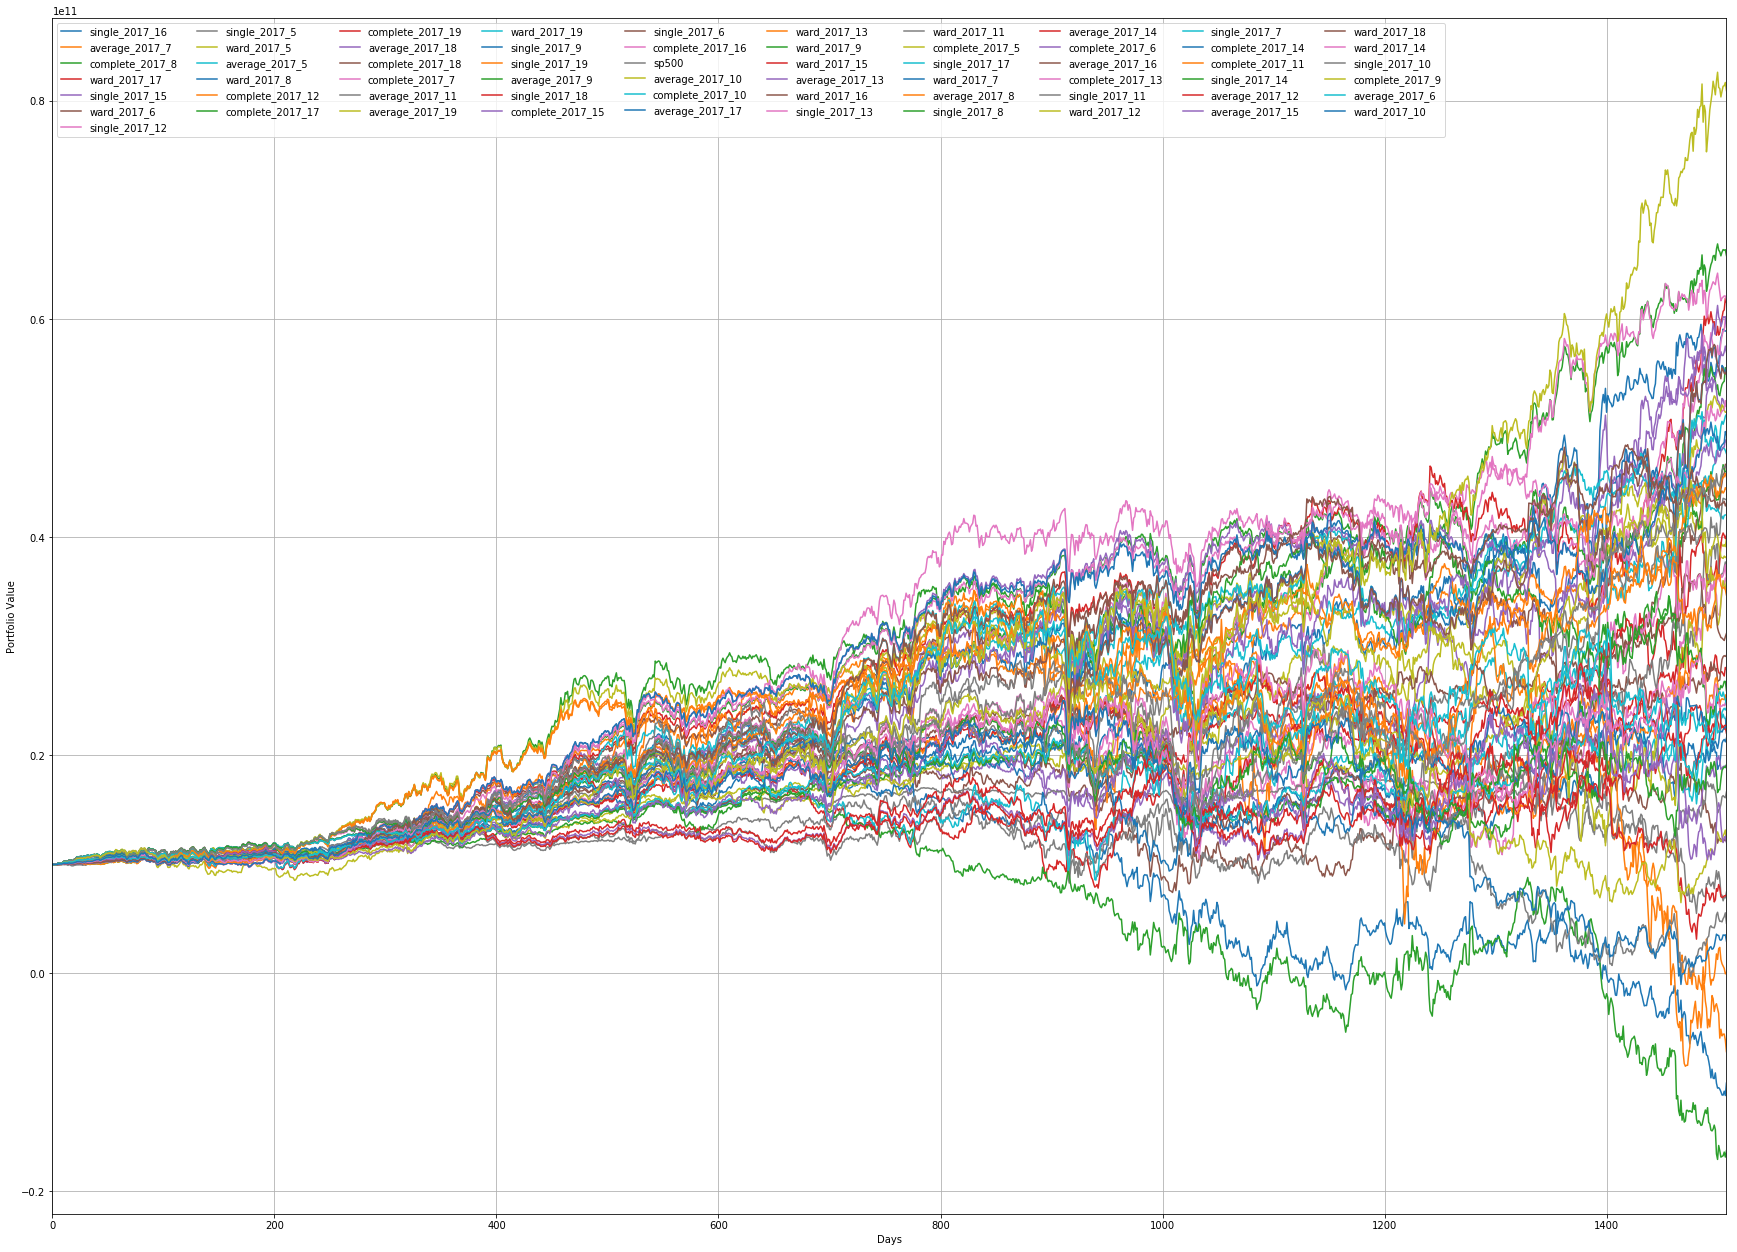
\includegraphics[width=\linewidth]{images/all_portfolio_return.png}
    \caption{Portfolio return for 60 candidate learned sector universes.}
    \label{fig:appendix_backtest:portfolio_return}
    \addcontentsline{toc}{section}{Portfolio Return}
\end{sidewaysfigure}

\newpage
\begin{sidewaysfigure}
    \centering
    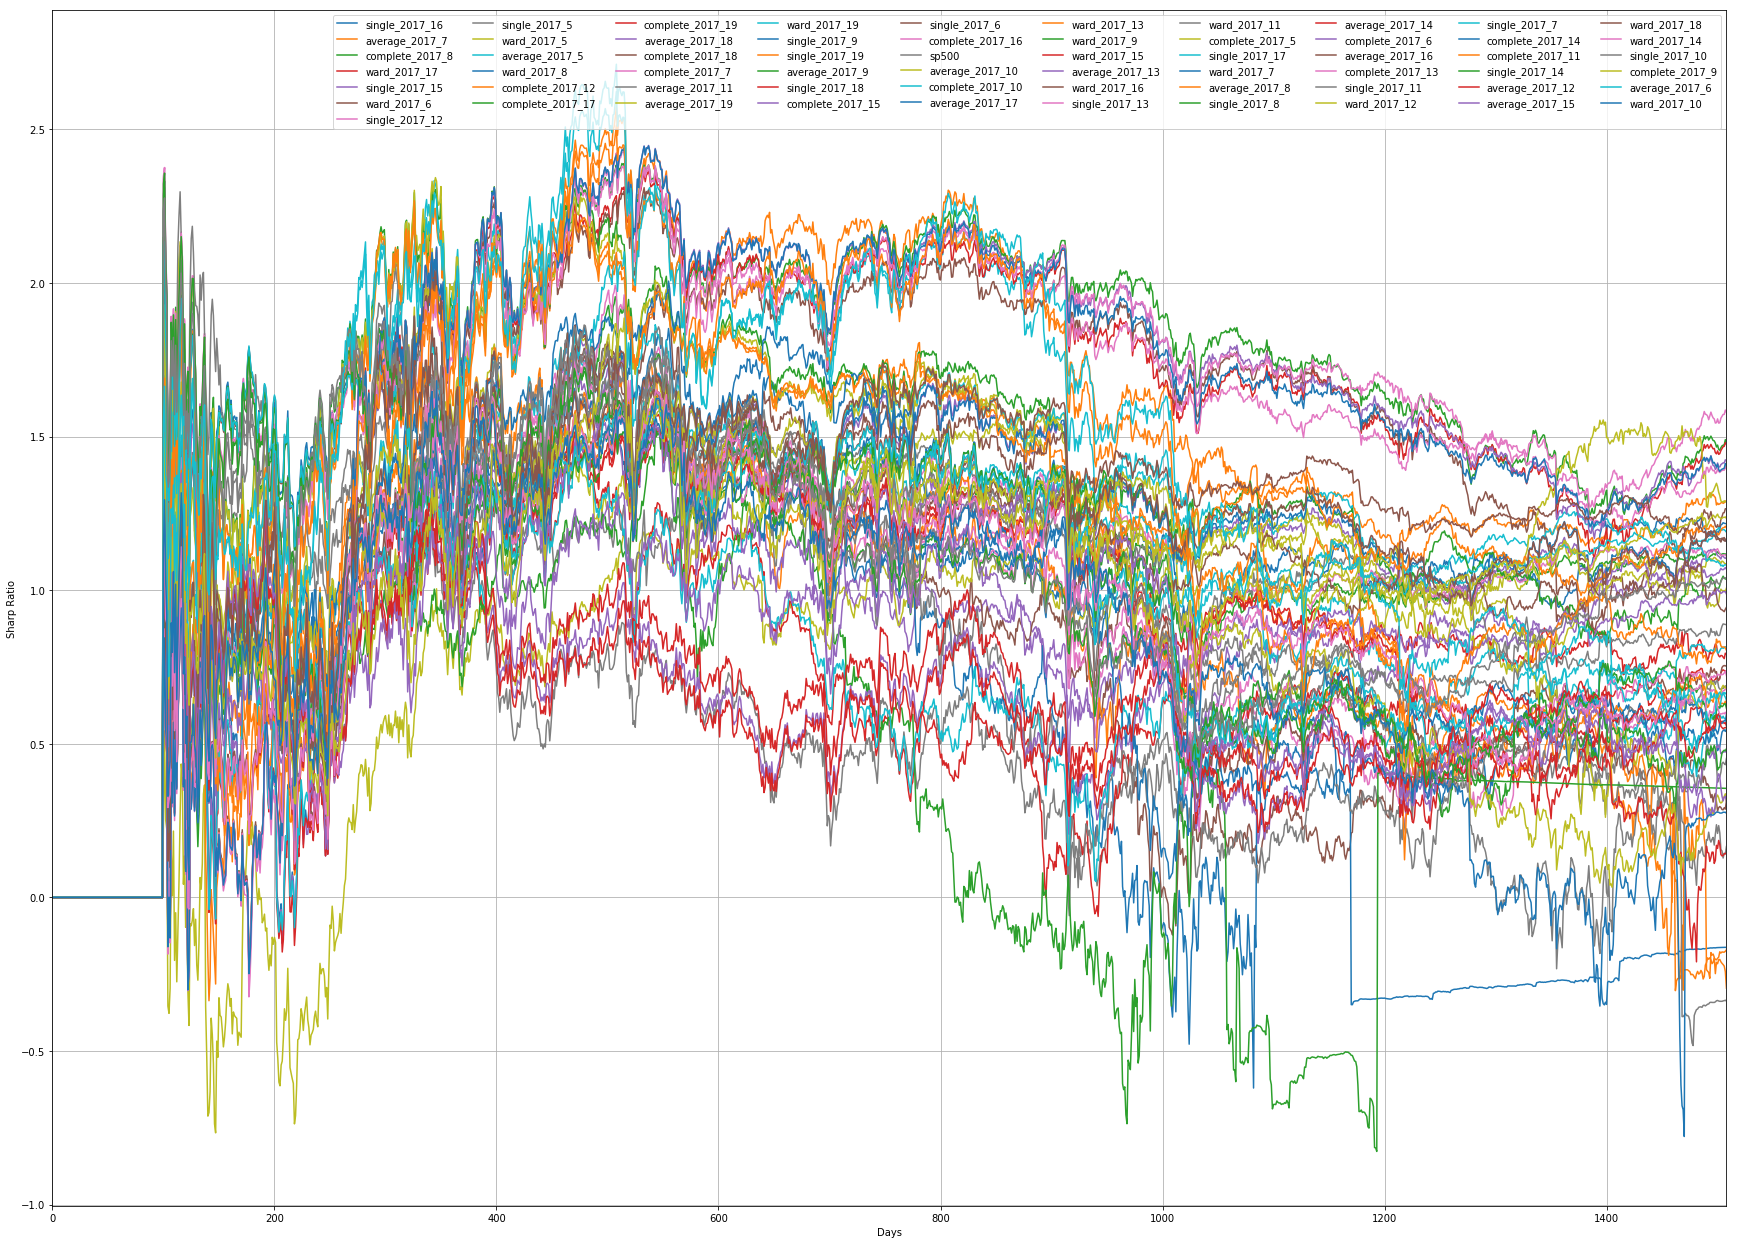
\includegraphics[width=\linewidth]{images/all_sharpe_ratio.png}
    \caption{Rolling Sharpe Ratio for 60 candidate learned sector universes.}
    \label{fig:appendix_backtest:sharpe_ratio}
    \addcontentsline{toc}{section}{Sharpe Ratio}
\end{sidewaysfigure}


\twocolumn

\chapter{Optimal Learned Sector Universe} \label{appendix:optimal_ls}

Put bar chart here

% Took forever to set up this table
% See: http://www.ctex.org/documents/packages/table/supertabular.pdf
% https://tex.stackexchange.com/questions/440078/how-can-i-generate-a-big-tabular-out-of-a-csv-file
% https://tex.stackexchange.com/questions/88387/disable-two-column-mode-for-separate-part
% https://tex.stackexchange.com/questions/269428/too-large-bottom-margin-with-xtab-or-supertabular
% https://latex.org/forum/viewtopic.php?t=5825
%
% Basically, supertabular over-estimates the page margins and causes a huge bottom margin to appear. To
% fix this the "\shrinkheight" command is run at each pagebreak (which is why its inserted into \tablehead)
% Had to seat first page height manually because this package is a mess
% Remember to add "showframe" option to geometry package when investigating this; figured out that it was
% messing up because the initial override I was setting was exceeding page margins

\clearpage


\begin{center}
    \tablefirsthead{%
        \shrinkheight{-0.5in}
        \hline
        \textbf{Ticker} & \textbf{GICS Sector} & \textbf{Learned Sector} \tabularnewline
        % \midrule
        \hline
    }
    \tablehead{%
        \shrinkheight{-0.9in}
        % \toprule
        \hline
        \textbf{Ticker} & \textbf{GICS Sector} & \textbf{Learned Sector} \tabularnewline
        % \midrule
        \hline
    }
    \tabletail{\midrule}
    \tablelasttail{\bottomrule}
    \begin{supertabular}{|c|c|c|}
        \csvreader[
            late after line=\\
        ]{report_data/complete_17_table.csv}{1=\ticker, 2=\gics, 3=\ls}{\ticker & \gics & \ls}
    \end{supertabular}
\end{center}



\onecolumn

\chapter{Backtest Portfolio Weights} \label{appendix:portfolio_weights}

\section*{Optimal Learned Sector Universe Portfolio}

See Figure~\ref{fig:appendix_weights:sharpe_optimal} on Page~\pageref{fig:appendix_weights:sharpe_optimal}.


\section*{Benchmark Sector Universe Portfolio}

See Figure~\ref{fig:appendix_weights:benchmark} on Page~\pageref{fig:appendix_weights:benchmark}.

\newpage
\begin{sidewaysfigure}
    \centering
    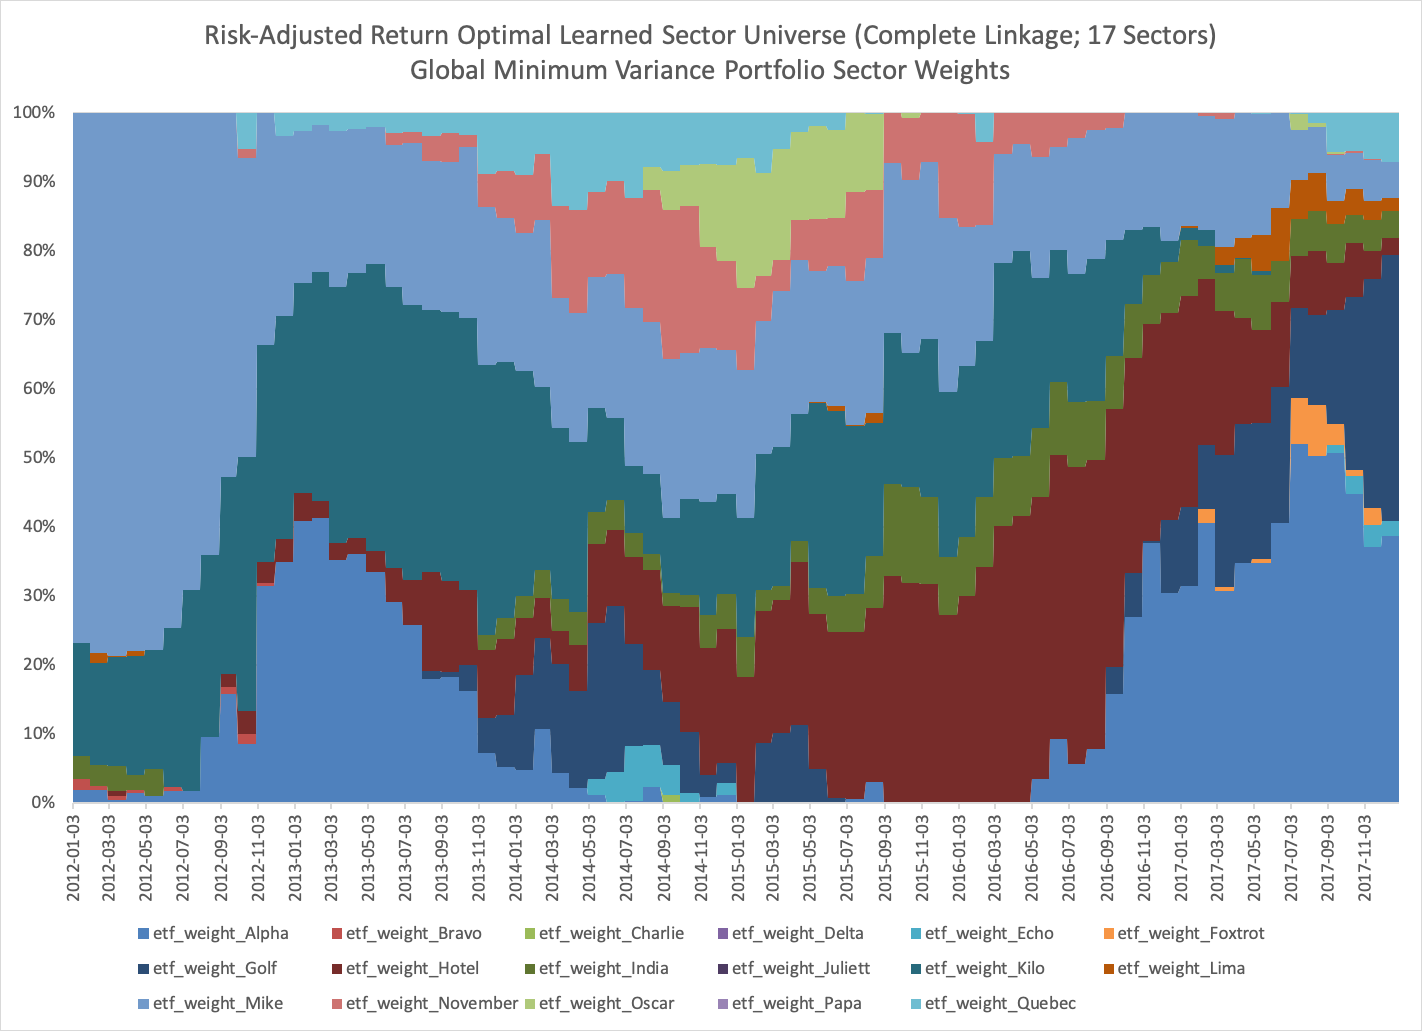
\includegraphics[width=\linewidth]{images/complete_17_sector_assignments.png}
    \caption{Risk-adjusted return optimal learned sector universe portfolio assignment weights.}
    \label{fig:appendix_weights:sharpe_optimal}
    \addcontentsline{toc}{section}{Optimal Learned Sector Universe Portfolio}
\end{sidewaysfigure}


\newpage
\begin{sidewaysfigure}
    \centering
    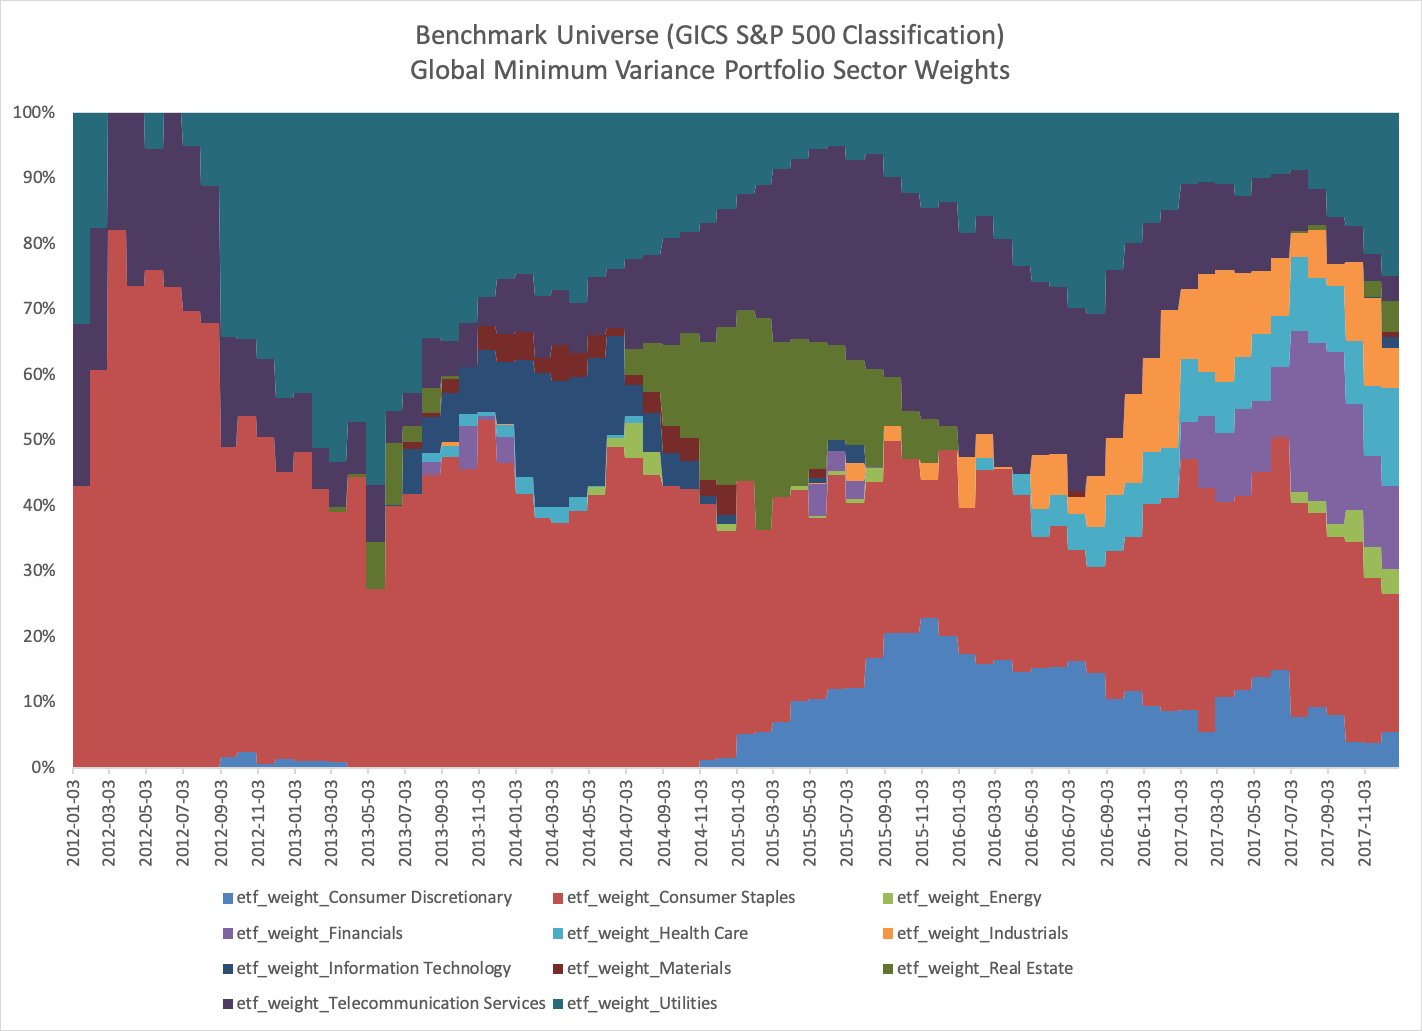
\includegraphics[width=\linewidth]{images/sp500_sector_assignments.png}
    \caption{Benchmark sector universe (i.e. \textit{GICS S\&P 500 Classification}) portfolio assignment weights.}
    \label{fig:appendix_weights:benchmark}
    \addcontentsline{toc}{section}{Benchmark Sector Universe Portfolio}
\end{sidewaysfigure}

\end{document}